\documentclass{article}

% Language setting
% Replace `english' with e.g. `spanish' to change the document language
\usepackage[polish]{babel}

% Set page size and margins
% Replace `letterpaper' with `a4paper' for UK/EU standard size
\usepackage[a4paper,top=2cm,bottom=2cm,left=3cm,right=3cm,marginparwidth=1.75cm]{geometry}

% Useful packages
\usepackage{polski}
\usepackage[utf8]{inputenc}
\usepackage{amsmath}
\usepackage{graphicx}
\usepackage[colorlinks=true, allcolors=blue,unicode]{hyperref}
\usepackage{courier}
\usepackage[T1]{fontenc}
\usepackage{lastpage}

\usepackage{fancyhdr}
\pagestyle{fancy}
\fancyhead[L]{Specyfikacja implementacyjna}
\fancyhead[C]{}
\fancyhead[R]{Kamil Fryszkowski, Oskar Biwejnis}
\cfoot{\thepage/\pageref{LastPage}}


\title{Specyfikacja implementacyjna projektu w języku Java}
\author{Kamil Fryszkowski, Oskar Biwejnis}

\begin{document}


\maketitle
\thispagestyle{fancy}
\section{Wstęp}
Celem projektu jest stworzenie programu w języku Java (wersja 1.8), posiadającego graficzny interfejs użytkownika, który będzie w stanie znajdować najkrótszą ścieżkę w pomiędzy dwoma wierzchołkami w danym grafie ważonym skierowanym. Użyte zostaną do tego algorytmy BFS oraz Dijkstry. Środowiskiem programistycznym będzie IntelliJ Idea (wersja 2022.1) wraz z pomocą narzędzia automatyzującego budowę oprogramowania Maven (wersja 3.8.5) i technologą JavaFX pozwalającą na wygodną pracę z graficznym interfejsem użytkownika. Wykorzystanym sposobem współpracy i wersjonowania jest system kontroli wersji GIT w domenie \texttt{\footnotesize projektor.ee.pw.edu.pl}. 


\section{Struktury danych}
Do poprawnego funkcjonowania programu niezbędne będzie użycie następujących struktur danych:
\begin{enumerate}
\item Do przechowywania grafu użyta zostanie struktura danych \texttt{Graph} zaimplementowana w bibliotekach Javy.
\item Kolejka FIFO użyta zostanie przy działaniu algorytmu BFS. W kolejce tej, pierwszy wprowadzony element będzie pierwszym wyjętym. Aplikacja korzystać będzie z kolejki zaimplementowanej w bibliotekach Javy.

\item Kolejka priorytetowa niezbędna będzie do poprawenego działania algorytmu Dijkstry. Priorytem według które będą wyjmowane elementy z kolejki będzie wartość \texttt{d[v]}, mówiąca o długości najkrótszej ścieżki do danego wierzchołka z wierzchołka startowego w danym momencie działania algorytmu. Aplikacja korzystać będzie z kolejki zaimplementowanej w bibliotekach Javy.

\end{enumerate}
\section{Tryby pracy programu}
    Program uruchamia się w jednym i głównym trybie działania, który pozwala na kliknięcie odpowiednich przycisków pozwalających na działanie w określonym zakresie. Dostępne przyciski to:
    \begin{enumerate}
    \item Tryby działania generatora
    \begin{itemize}
        \item RandWeightMode - pozwala na stworzenie grafu, w którym istnieją wszystkie krawędzie
        zawierające się w danym przedziale wierzy i kolumn z wygenerowanymi losowo z danego przedziału wagami
        \item AllRandMode - pozwala na stworzenie grafu, w którym istnieje jedynie określona szansa
        na powstanie danej krawędzi
        \item  ConMode - działa jak AllRandMode, jednak graf generuje się tak długo, aż nie będzie spójny.
    \end{itemize}
    \item Wyświetlanie grafu
    \begin{itemize}
        \item Koloruj wagi - pozwala na graficzne odwzorowanie wag według koloru (najmniejsze wagi - najjaśniejszy kolor)
        \item Wyswietl jedynie krawędzie ścieżki - wyłącza wyświetlanie tych krawędzi, przez które nie prowadzi ścieżka
        
    \end{itemize}
    \item Obsługa piliku
    \begin{itemize}
        \item Zapisz do pliku - zapisuje graf do pliku
        \item Wczytaj z pliku - wczytuje graf z pliku
    \end{itemize}
    \item Wyszukiwanie ścieżki i badanie spójności
    \begin{itemize}
        \item Szukaj - po podaniu dwóch wierzchołków znajduje najkrótszą ścieżkę między nimi
        \item Sprawdź spójność - sprawdza czy graf jest spójny
    \end{itemize}
    
\end {enumerate}

\section{Modularna struktura programu}
\begin{figure}[htp]
\centering
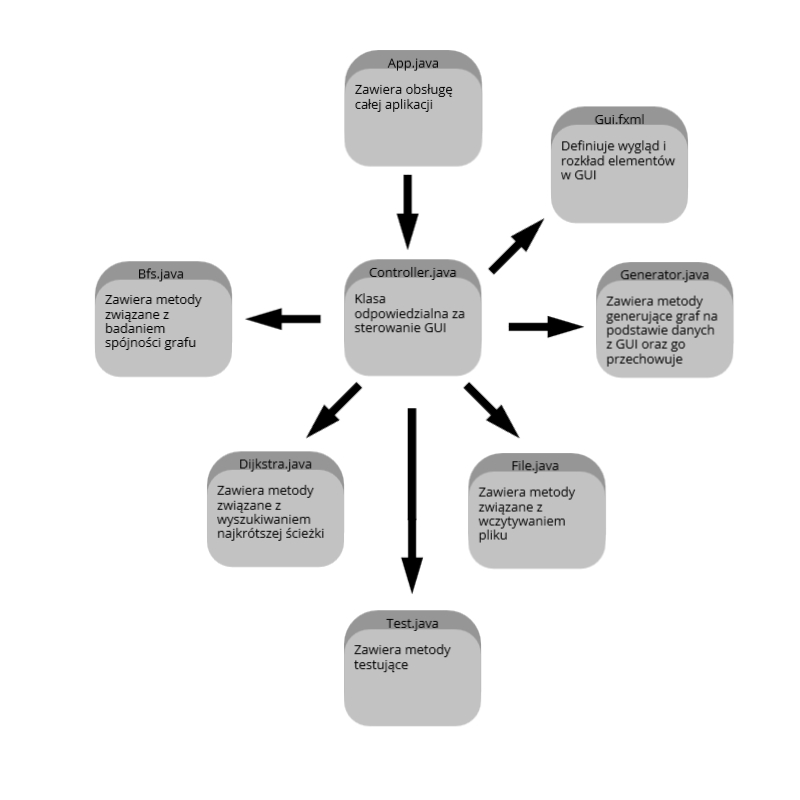
\includegraphics[width=0.9\textwidth]{moduly.jpeg}
\caption{\label{fig:mod}Graficzna reprezentacja struktury programu (opracowanie własne)}
\end{figure}

\begin{itemize}
    

\item App.java:
    \begin{itemize}
        
    
    \item \texttt{\footnotesize void main(String[] args)} – odpowiada za całe sterowanie programem
    
    
    \end{itemize}
    
\item Generator.java:
    \begin{itemize}
    \item \texttt{\footnotesize Graph graph} - struktura przechowująca graf
    \item \texttt{\footnotesize void findNeighbours (Graph graph, int vertex, int rows, int cols, double minWeight, double maxWeight)} - odpowiada za szukanie sąsiadów poszczególnych wierzchołków
   
    \item \texttt{\footnotesize Graph generateRandWeightMode (int rows, int cols, double minWeight, double maxWeight)} - odpowiada za generowanie grafu typu "kartka w kratkę"
    \item \texttt{\footnotesize Graph generateAllRandMode (int rows, int cols, double minWeight, double maxWeight)} - odpowiada za generowanie losowego grafu
    \item \texttt{\footnotesize Graph generateConMode (int rows, int cols, double minWeight, double maxWeight)} - odpowiada za generowanie spójnego grafu
    \end{itemize}
\item Bfs.java:
    \begin{itemize}
    \item \texttt{\footnotesize Queue<Integer> queue} – struktura kolejki dla algorytmu BFS
    \item \texttt{\footnotesize int BFS(Graph graph, int n, int startingVertex)} – odpowiada za działanie algorytmu BFS
    \item \texttt{\footnotesize String isConst(Graph graph, int rows, int columns)} – odpowiada za sprawdzenie, czy graf jest spójny oraz zwraca odpowiedni komunikat
    \end{itemize}
\item Controller.java:
    \begin{itemize}
    \item \texttt{\footnotesize void gui()} – odpowiada za obsługę graficznego interfejsu użytkownika
    \item \texttt{\footnotesize void printComunicate(String)} – odpowiada za wypisanie podanego tekstu w okienku komunikatów
    \end{itemize}
\item Dijkstra.java:
    \begin{itemize}
    \item \texttt{\footnotesize PriorityQueue<Double> pQueue} – struktura kolejki priorytetowej dla algorytmu Dijkstry
     \item \texttt{\footnotesize LinkedList<Integer> path} – struktura listy liniowej dla najkrótszej ścieżki
    \item \texttt{\footnotesize String printPath(Graph graph, LinkedList<Integer> path, boolean doPrintWeights)} – zwraca tekst komunikatu zawierającego wypisaną najkrótszą ścieżkę 
    \item \texttt{\footnotesize LinkedList<Integer> dijkstra (Graph graph, int start, int destination, int rows , int cols)} – odpowiada za działanie algorytmu dijkstry, zwraca listę liniową z kolejnymi wierzchołkami w najkrótszej ścieżce
    \end{itemize}

\item File.java:
    \begin{itemize}
    \item \texttt{\footnotesize Graph readFile (String filePath)} - odpowiada za czytanie grafu z pliku
    \item \texttt{\footnotesize void printGraphToFile (Graph graph, int rows, int cols)} - odpowiada za zapisywanie grafu do pliku
    \end{itemize}

\item Test.java - zawiera w sobie testy opisane szerzej w punkcie 7.
   
    
    
    
\item Gui.fxml - definiuje wygląd, funkcjonalności i rozmieszczenie elementów w graficznym interfejsie użytkownika
    
\end{itemize}


\section{Algorytm BFS}
Działanie algorytmu BFS, czyli algorytmu przeszukiwania grafu wszerz, można streścić następująco: \\ \\
Wybieramy wierzchołek startowy. Następnie odwiedzamy po kolei wszystkie wierzchołki sąsiadujące z wierzchołkiem startowym. Następnie odwiedzamy po kolei wszystkie nieodwiedzone wierzchołki sąsiadujące z wierzchołkami sąsiadującymi z wierzchołkiem startowym i tak dalej…\\
Niezbędna do funkcjonowania BFSa jest kolejka FIFO (patrz pkt 2.) oraz tablica która dla każdego wierzchołka będzie posiadała informację o jego stanie: \\

0  – nieodwiedzony (kolor biały) \\
1 – dodany do kolejki lecz nieodwiedzony (kolor szary) \\
2  - odwiedzony (kolor czarny) \\

\textbf{Złożoność pamięciowa}
 \\Dla wykorzystanej w tym programie listy sąsiedztwa złożoność pamięciowa opisana jest wzorem O(V+E) gdzie: V - liczba wierzchołków, E - liczba krawędzi.\\

\textbf{Złożoność czasowa}
\\Pesymistyczny przypadek to taki, gdy algorytm musi odwiedzić wszystkie wierzchołki oraz krawędzie, wtedy złożoność czasowa wynosi O(V+E), gdzie V - liczba wierzchołków, E - liczba krawędzi.
\section{Algorytm Dijkstry}
Algorytm dijkstry służy do znajdowania  \textbf{najkrótszej ścieżki} w grafie ważonym. Przez \textbf{ścieżkę} pomiędzy dwoma wierzchołkami rozumiemy kolejno uporządkowane wierzchołki, które należy odwiedzić aby dostać się z wierzchołka startowego do końcowego. Z kolei \textbf{najkrótszą} ścieżką jest ta, której suma wag krawędzi jest najniższa. Algorytm Dijkstry, podczas działania, znajduje najkrótsze ścieżki do każdego wierzchołka do którego można dojść z wierzchołka startowego
\\ \\
Niezbędne do poprawnego działania będzie utworzenie:
\begin {itemize}

\item Tablicy d[V], gdzie V oznacza liczbę wszystkich wierchołków w grafie. Przechowywać będzie ona informację o długości aktualnej najkrótszej ścieżki z wierzchołka startowego do danego wierzchołka. Dla wierzchołka startowego s, d[s] przyjmuje początkowo wartość 0, a dla każdego innego nieskończoność.
\item Tablicy p[V], gdzie V oznacza liczbę wszystkich wierchołków w grafie. Przechowywać będzie ona informację o poprzednim wierzchołku w najkrótszej ścieżce do danego wierzchołka. Początkowo jest pusta.
\item Kolejki priorytetowej opartej na strukturze kopca. W kolejce tej początkowo będą wszystkie wierzchołki, a priorytetem wyciągania elementów z niej będzie najniższa wartość d[v] dla danego wierzchołka v.\\

\end{itemize}

\section{Testowanie}
Poprawność działania programu należy sprawdzić kolejno testami, oraz wyniki porównać z wcześniej przygotowanymi danymi:
\begin{itemize}
    \item \texttt{int testAllRandModeGenerator()} - funkcja sprawdzająca poprawność działania generator w trybie AllRandMode
    \item \texttt{int testRandWeightModeGenerator()} - funkcja sprawdzająca poprawność działania generator w trybie RandWeightMode
    \item \texttt{int testConModeGenerator()} - funkcja sprawdzająca poprawność działania generator w trybie ConMode
    \item \texttt{int testBFS()} - funkcja sprawdzająca poprawność działania algorytmu BFS
    \item \texttt{int testDijkstra()} - funkcja sprawdzająca poprawność działania algorytmu Dijkstry 
    \item \texttt{int testRead()} - funkcja sprawdzająca poprawność działania wczytywania grafu z pliku
    \item \texttt{int testSave()} - funkcja sprawdzająca poprawność działania zapisywania grafu do pliku

\end{itemize}

\section{Źródła}
\begin{enumerate}
    \item https://pl.wikipedia.org
\end{enumerate}


\end{document}
